\documentclass{standalone}

\usepackage{tikz}
  \usetikzlibrary{positioning}
  \usetikzlibrary{arrows.meta}
  \usetikzlibrary{arrows, shapes, trees, positioning, decorations.markings, patterns}
  \usetikzlibrary{backgrounds,fit,decorations.pathreplacing}
  \usetikzlibrary[topaths]
  % \usetikzlibrary[graphdrawing] %% only luatex
% \usepackage[active,tightpage]{preview}
\usepackage{tikz-bpmn}
\usepackage{bpmn-gateways}
\usepackage{bpmn-events}
\usepackage{tikzpeople}

\usepackage{fontspec}
  \setmainfont[Ligatures=TeX]{Nimbus Roman No9 L}

\usepackage{graphicx}
\graphicspath{{}{./assets/}}

\begin{document}

\begin{tikzpicture}[node distance=1.5cm]

  \tikzset{
    ->,
    >=stealth',
    font={\fontsize{11pt}{12}\selectfont}
  }

  \tikzstyle{surround} = [fill=white!10,very thick,draw=black,rounded corners=2mm]

  % \node[task] (custA) {
\includegraphics{account_box} \\ Customer A \\ Debtor};

% \node[draw,rectangle,minimum size=1.5cm] at (0,2) {};
  \node[] (merch3) at (1,10) {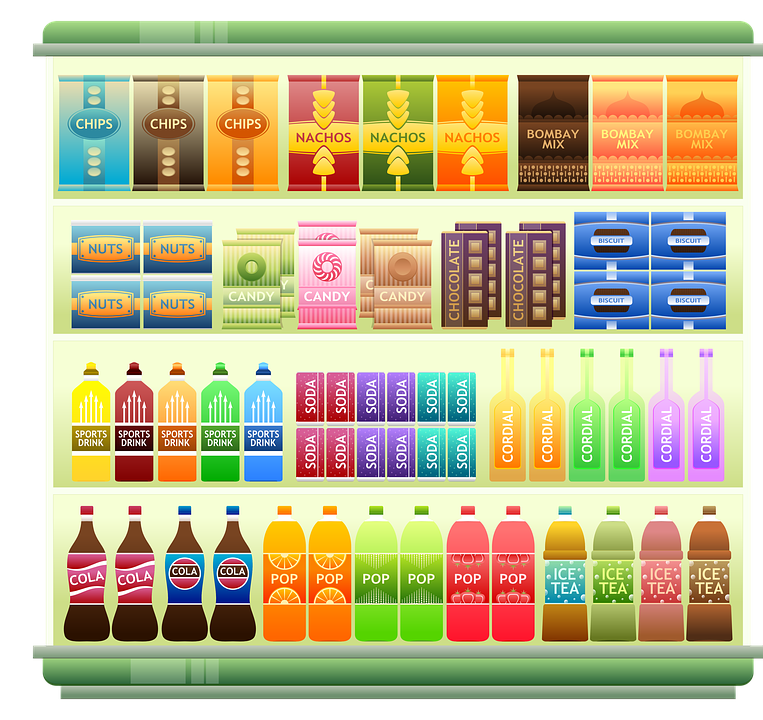
\includegraphics[scale=0.07]{supermarket-shelf-1}};
  \node[bob,minimum size=0.5cm,right of=merch3] (cust3) {};
  \node[businessman,minimum size=0.5cm,right of=cust3, node distance=5cm] (cust1) {};
  \node[right of=cust1] (qr) {\includegraphics[scale=0.4]{qrcode}};
  \node[right of=qr] (merch1) {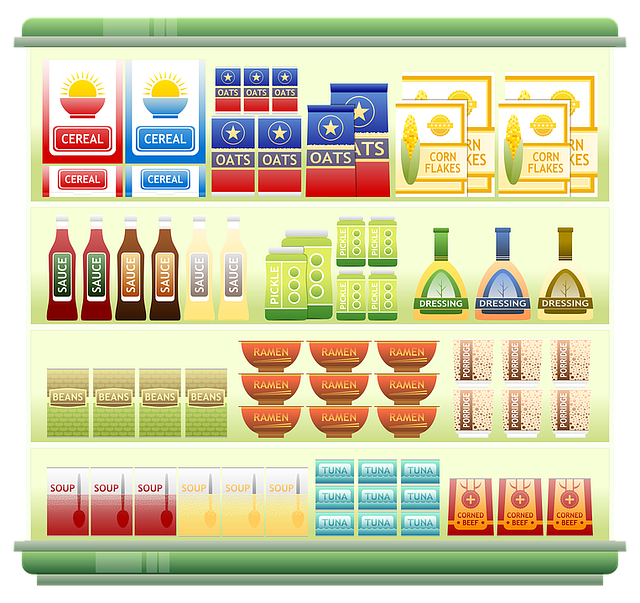
\includegraphics[scale=0.08]{supermarket-shelf-2}};
  % \node (cart1) at (9, 10) {\includegraphics[scale=0.03]{cart}};
  % \node[surround] (a1) {};
  % \node (a2) at (8, 5) {};
  \node[surround] (m1) at (6, 9) [text width=2cm, font={\fontsize{7pt}{12}\selectfont}, minimum height=3.5cm] {\textbf{Shopping Cart:} \\ - Item1 \\ - Item2 \\ - Item3 \\ Total: 100};
  \node (i1) at (7, 7.6) {};
  \draw (qr) edge[bend left] node{} (m1.east); 
  \node[charlie,minimum size=0.5cm, below of=cust3, node distance=7cm] (cust4)  {};
  \node[below of=merch3, node distance=7cm] (merch4) {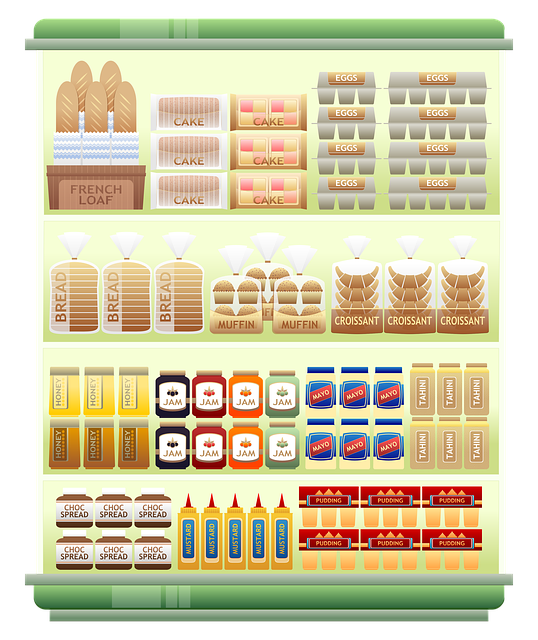
\includegraphics[scale=0.08]{supermarket-shelf-3}};
  \node[alice,minimum size=0.5cm,below of=qr, node distance=7cm] (cust2) {};
  \node[below of=merch1, node distance=7cm] (merch2) {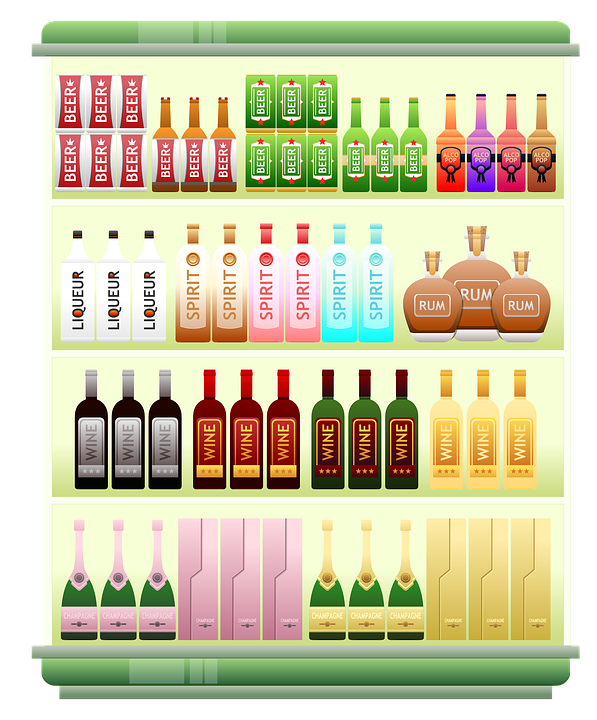
\includegraphics[scale=0.08]{supermarket-shelf-4}};

  % \node (b1) at (2, 4) {};
  % \node (b2) at (4, 0) {};

  % \node (pos1) at (3, -1) {};
  % \node (pos2) at (7, -1) {};
  \node[surround] (m2) at (4, 4) [text width=2cm, font={\fontsize{7pt}{12}\selectfont}, minimum height=3.5cm] {\textbf{Checkout:} \\ - Item1 \\ - Item2 \\ - Item3 \\ Total: 100 \\ Payment methods: \\ 
\includegraphics[scale=0.02]{ethereum} 
\includegraphics[scale=0.02]{bitcoin} 
\includegraphics[scale=0.02]{litecoin}};
  \node[surround] [right of=m2,node distance=2cm, fill=blue!10, text width=1.4cm] (pos) at (4, 3) {
\includegraphics[scale=0.03]{nfc} NFC Terminal};
  % \draw (m2) edge[bend left] node{} (pos); 

  % \node (payzone) at (5, -1) {Payment Zone};

  % \node (phone) at (5,5) {Smart Phone Screen};

\begin{pgfonlayer}{background}
        % Compute a few helper coordinates
        \path (merch3.west |- merch1.north)+(-0.5,0.3) node (a) {};
        \path (merch2.south -| merch2.east)+(+0.3,-0.2) node (b) {};
        \path[fill=yellow!10,rounded corners, draw=black!50]
            (a) rectangle (b);
        % \path (pos1.west |- pos1.north)+(-0.5,0.3) node (p1) {};
        % \path (pos2.south -| pos2.east)+(+0.3,-0.2) node (p2) {};
        % \path[fill=yellow!20,rounded corners, draw=black!50, dashed]
            % (p1) rectangle (p2);
        % \path (gyros.north west)+(-0.2,0.2) node (a) {};
        % \path (IMU.south -| gyros.east)+(+0.2,-0.2) node (b) {};
    \end{pgfonlayer}

% \begin{pgfonlayer}{background} 
  % \node[surround] (background) [fit = (a1) (a2)] {};
  % \node[surround] (background) [fit = (b1) (b2)] {};
% \end{pgfonlayer}

\end{tikzpicture}

\end{document}
